\chapter{APPLICATION NUMERIQUE}
\thispagestyle{empty}

\section{Cost Analysis}

This section presents a detailed cost analysis of the project, considering all resources that contribute to the realization of the system. Following the guidelines, both economic resources and computational resources are accounted for.

\subsection{Computational Resources}

The primary computational resources are summarized in Table~\ref{tab:compute-resources}.

\begin{table}[htbp]
\centering
\caption{Computational resources used in the project.}
\label{tab:compute-resources}
\begin{tabular}{llr}
\toprule
\textbf{Resource} & \textbf{Specification} & \textbf{Quantity} \\
\midrule
GPU & NVIDIA RTX 4070 Laptop (8GB VRAM) & 1 \\
CPU & AMD Ryzen 9 8945HS (4GHz) & 1 \\
RAM & DDR5 32GB & 32 GB \\
Storage & NVMe SSD & 512 GB \\
\bottomrule
\end{tabular}
\end{table}

\subsection{Dataset Sizes}

The dataset sizes for the Custom-WikiCS collection are presented in Table~\ref{tab:dataset-sizes}.

\begin{table}[htbp]
\centering
\caption{Dataset storage requirements.}
\label{tab:dataset-sizes}
\begin{tabular}{lr}
\toprule
\textbf{Component} & \textbf{Size} \\
\midrule
WikiCS raw data (PyG format) & 202.2 MB \\
BGE-M3 embeddings (11,367 $\times$ 1024 $\times$ float32) & 21.3 MB \\
Node2Vec embeddings (11,367 $\times$ 128 $\times$ float32) & 6.5 MB \\
Combined embedding cache & 27.8 MB \\
Adjacency matrix (sparse) & 8.2 MB \\
Total & \multicolumn{1}{r}{238.2 MB} \\
\bottomrule
\end{tabular}
\end{table}

The raw WikiCS graph data dominates the storage footprint at 202.2 MB, while the combined embedding cache accounts for only 27.8 MB (~12\% of total). Pre-computing embeddings offline saves significant recomputation time.

\subsection{GPU Memory Usage}

GPU memory requirements vary by model and configuration, as shown in Table~\ref{tab:gpu-memory}.

\begin{table}[htbp]
\centering
\caption{GPU memory usage by model configuration.}
\label{tab:gpu-memory}
\begin{tabular}{lrr}
\toprule
\textbf{Model} & \textbf{Configuration} & \textbf{GPU Memory} \\
\midrule
GCN & 2 layers, 128 hidden units & 2--3 GB \\
GAT & 2 layers, 8 heads, 128 hidden units & 4--6 GB \\
BGE-M3 inference (batch) & 11,367 nodes & 3--4 GB \\
Combined (training) & GAT + embeddings on GPU & 6--8 GB \\
\bottomrule
\end{tabular}
\end{table}

The RTX 4070's 8GB VRAM is sufficient for all current experiments but leaves limited headroom for larger batch sizes or more complex models.

\subsection{Training Time}

Table~\ref{tab:training-time} presents estimated training times for different configurations on the RTX 4070 Laptop.

\begin{table}[htbp]
\centering
\caption{Training time estimates for 100 epochs.}
\label{tab:training-time}
\begin{tabular}{lrr}
\toprule
\textbf{Model} & \textbf{Time per Epoch} & \textbf{Total (100 epochs)} \\
\midrule
GCN (baseline) & 8--12 sec & 13--20 min \\
GAT (2 layers, 4 heads) & 15--25 sec & 25--40 min \\
GAT (3 layers, 8 heads) & 30--45 sec & 50--75 min \\
\bottomrule
\end{tabular}
\end{table}

The current GCN baseline experiment (100 epochs) completes in approximately 15--20 minutes on the available hardware.

\subsection{Embedding Generation Time}

Table~\ref{tab:embedding-time} presents the time required for generating sentence embeddings.

\begin{table}[htbp]
\centering
\caption{Embedding generation times.}
\label{tab:embedding-time}
\begin{tabular}{lrr}
\toprule
\textbf{Model} & \textbf{Time (11,367 articles)} & \textbf{Hardware} \\
\midrule
BAAI/bge-m3 (1024-dim) & 30--60 min & RTX 4070 GPU \\
mGTE-modernbert (768-dim) & 20--40 min & RTX 4070 GPU \\
SVD-Node2Vec (128-dim) & 2--5 min & CPU \\
\bottomrule
\end{tabular}
\end{table}

BGE-M3 embedding generation is a one-time cost; embeddings are cached for subsequent experiments.

\subsection{Power Consumption}

Table~\ref{tab:power-consumption} presents power consumption estimates.

\begin{table}[htbp]
\centering
\caption{Power consumption per training run.}
\label{tab:power-consumption}
\begin{tabular}{lrr}
\toprule
\textbf{Component} & \textbf{Power Draw} & \textbf{Duration (GCN training)} \\
\midrule
GPU (RTX 4070) & 300W (peak) / 150W (avg) & 15--20 min \\
System (CPU, RAM, SSD) & 100W & 15--20 min \\
Total & 200--400W (avg ~250W) & 15--20 min \\
\midrule
\textbf{Energy per Run} & \multicolumn{2}{c}{0.06--0.10 kWh} \\
\bottomrule
\end{tabular}
\end{table}

Assuming 20 complete training runs (hyperparameter exploration, ablation studies), the total energy consumption for GNN training is approximately 1.2--2.0 kWh.

\subsection{Human Resources}

Table~\ref{tab:human-resources} presents the estimated human effort for the project.

\begin{table}[htbp]
\centering
\caption{Human effort estimates (hours).}
\label{tab:human-resources}
\begin{tabular}{lr}
\toprule
\textbf{Activity} & \textbf{Hours} \\
\midrule
Literature survey & 60 hours \\
Dataset construction (Custom-WikiCS) & 40 hours \\
Embedding generation and caching & 10 hours \\
Graph analysis (Report-4) & 30 hours \\
GNN model implementation and training & 50 hours \\
Recommendation system development (Report-5) & 40 hours \\
Report writing (all mid-reports + final) & 80 hours \\
\midrule
\textbf{Total} & \textbf{310 hours} \\
\bottomrule
\end{tabular}
\end{table}

\section{First Results}

This section presents the initial experimental results obtained to date.

\subsection{Graph Structural Analysis}

Prior to model development, a comprehensive structural analysis of the Custom-WikiCS graph was performed (Report-4). Key findings are summarized below.

\begin{figure}[H]
    \centering
    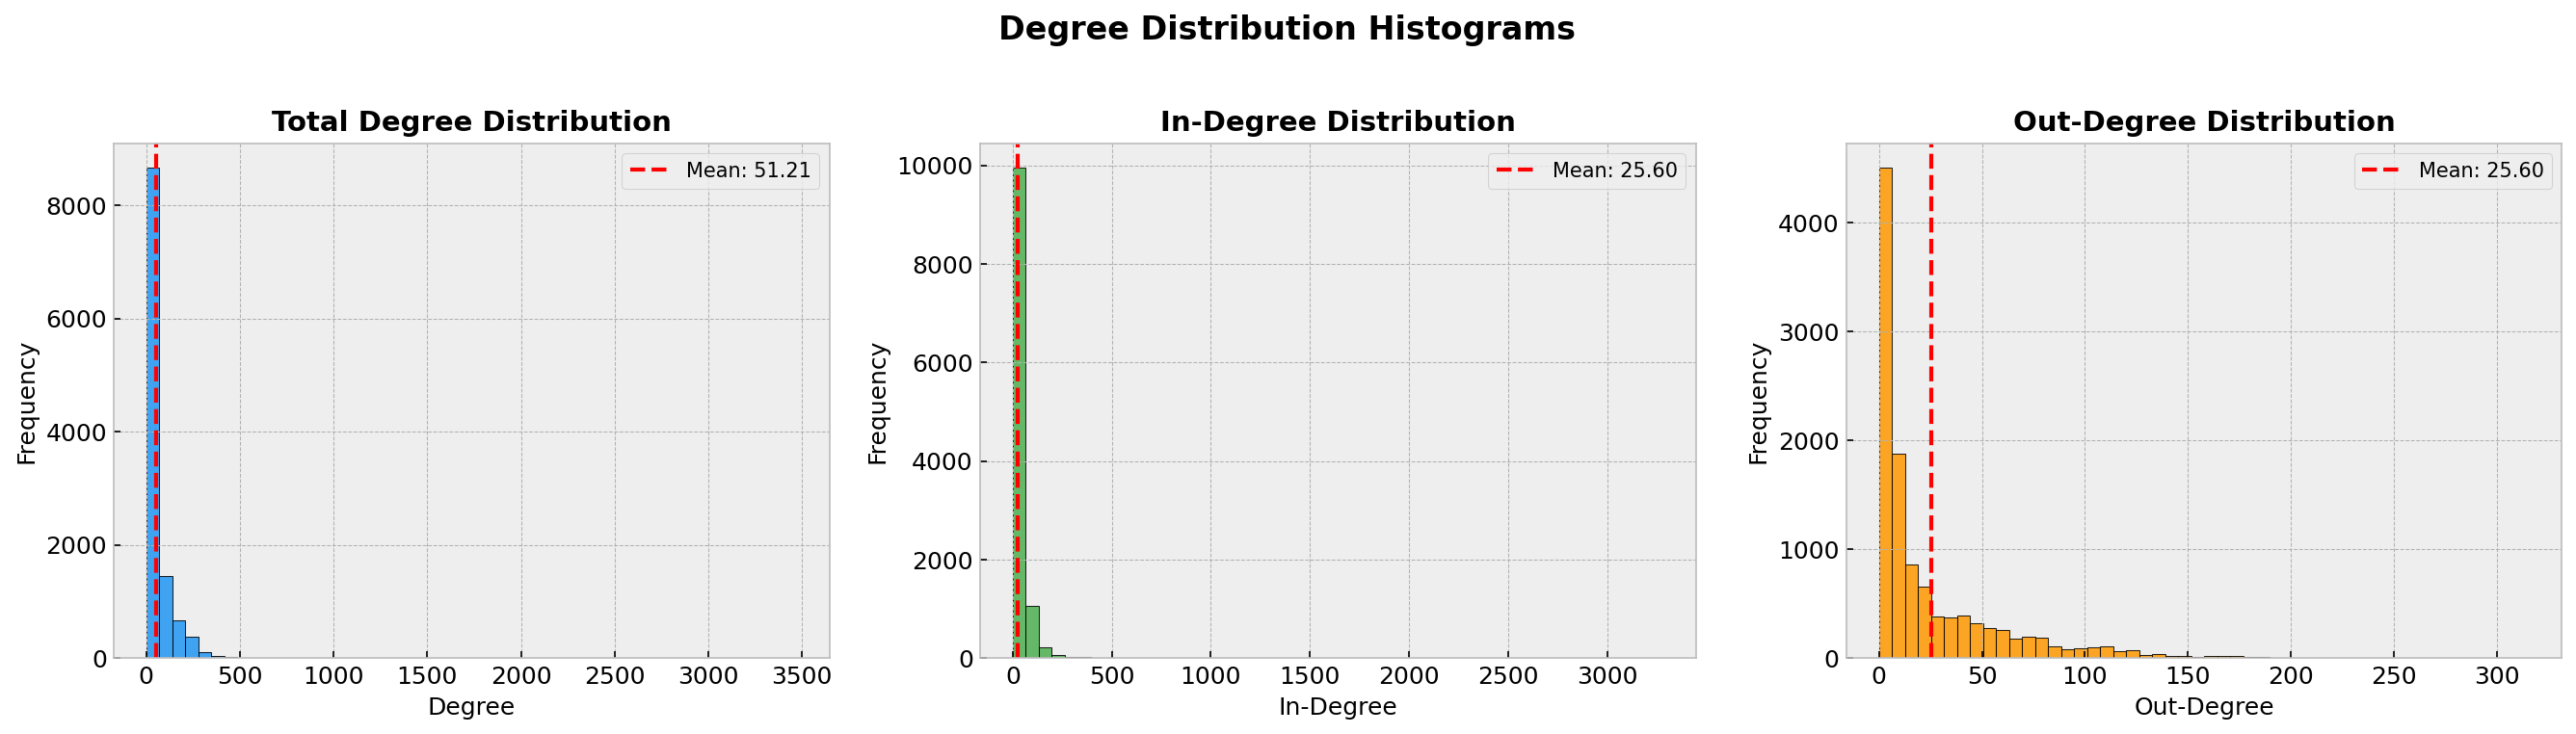
\includegraphics[width=0.75\textwidth]{figures/degree-distribution.png}
    \caption{Degree distribution of the cleaned Custom-WikiCS graph.}
    \label{fig:degree-dist}
\end{figure}

The degree distribution (Figure~\ref{fig:degree-dist}) follows a power-law pattern, characteristic of scale-free networks. Table~\ref{tab:degree-stats} presents the degree statistics.

\begin{table}[htbp]
\centering
\caption{Degree statistics for the cleaned graph.}
\label{tab:degree-stats}
\begin{tabular}{lrrrr}
\toprule
 & \textbf{Min} & \textbf{Max} & \textbf{Mean} & \textbf{Median} \\
\midrule
Total Degree & 1 & 3,474 & 51.21 & 16 \\
In-Degree & 0 & 3,283 & 25.60 & 4 \\
Out-Degree & 0 & 316 & 25.60 & 10 \\
\bottomrule
\end{tabular}
\end{table}

\begin{figure}[H]
    \centering
    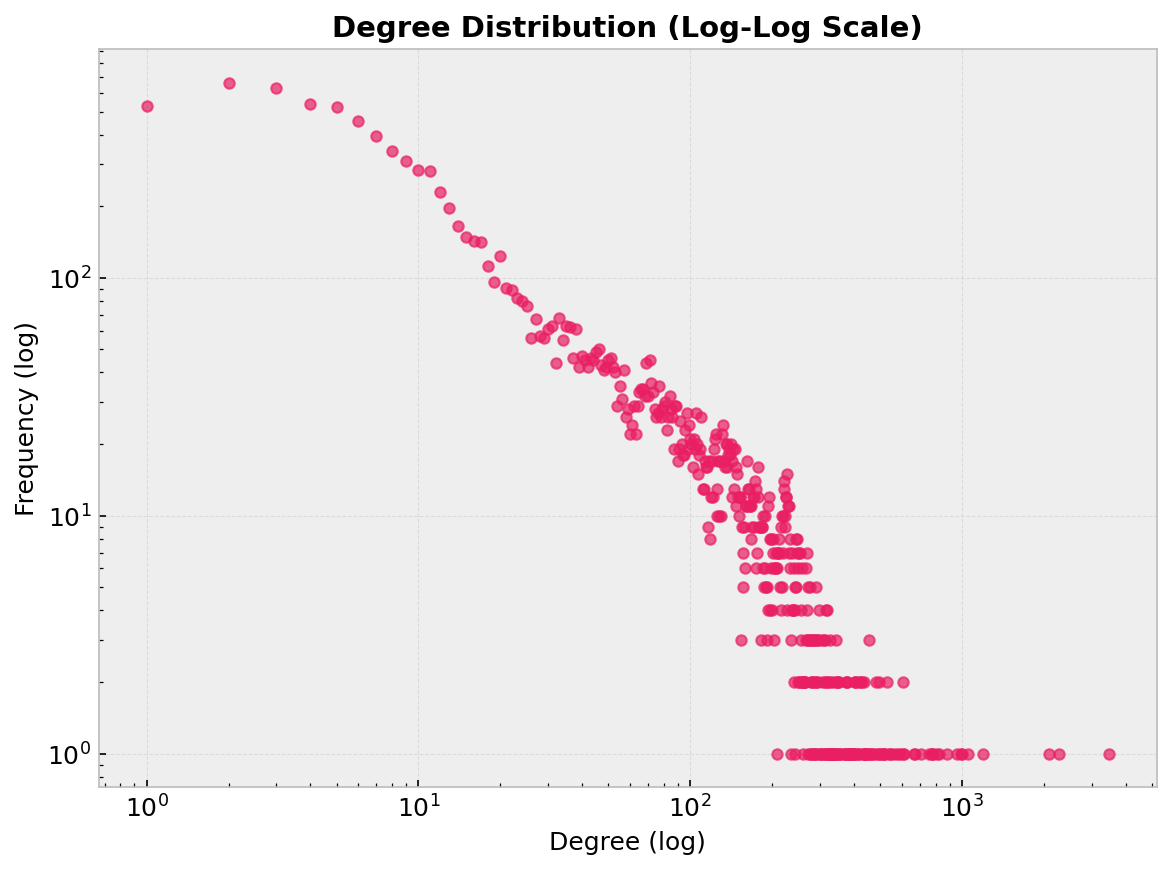
\includegraphics[width=0.65\textwidth]{figures/degree-log-log.png}
    \caption{Degree distribution on log-log scale (power-law assessment).}
    \label{fig:degree-loglog}
\end{figure}

The approximately linear relationship on log-log axes (Figure~\ref{fig:degree-loglog}) confirms the power-law behavior, with the fitted exponent $\alpha \approx 3.0$.

\begin{figure}[H]
    \centering
    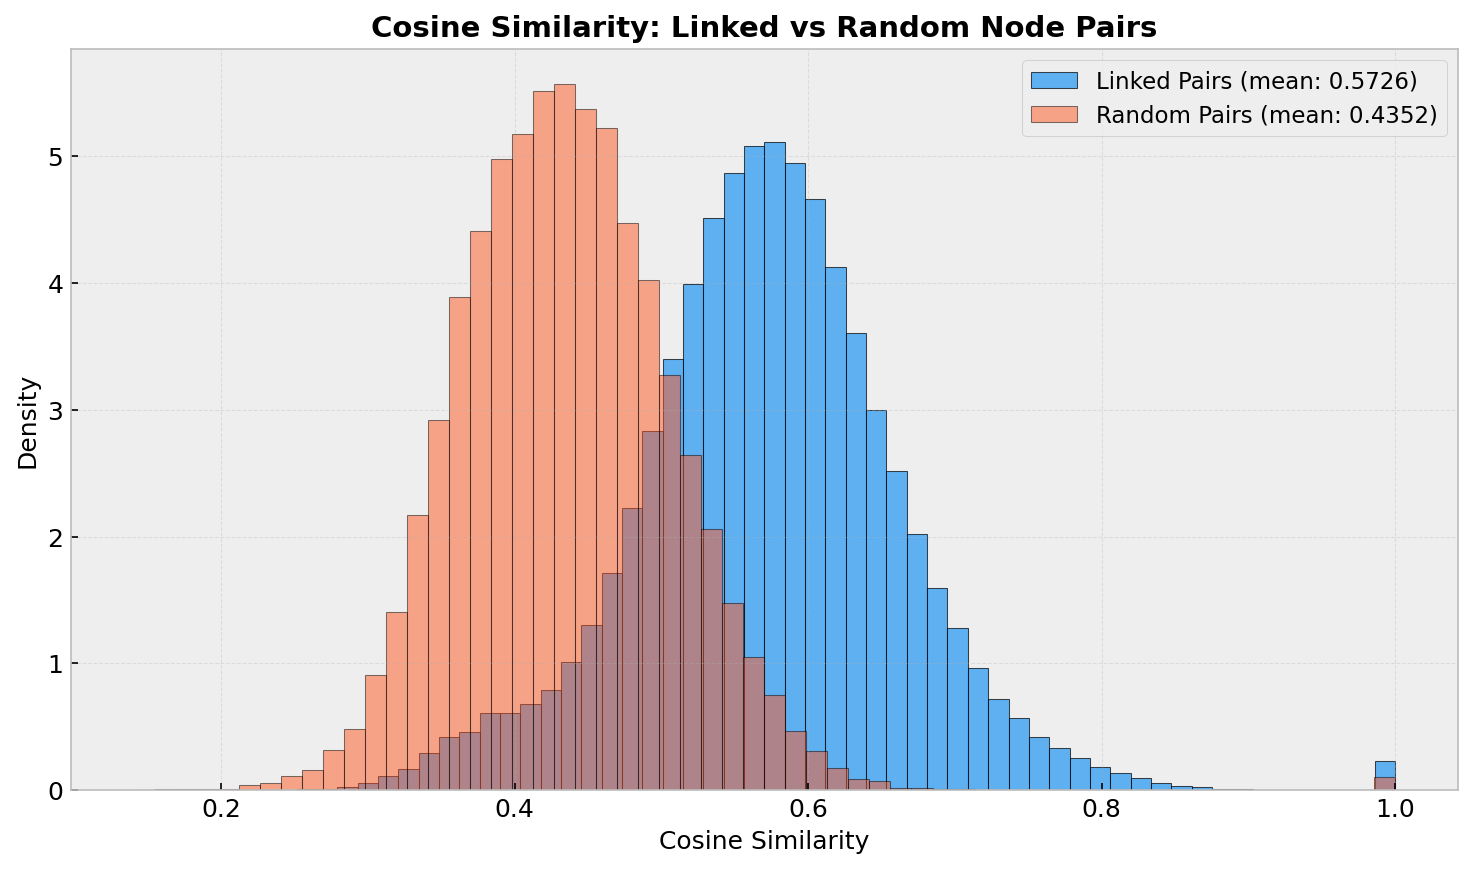
\includegraphics[width=0.75\textwidth]{figures/cosine-similarity-assortativity.png}
    \caption{Cosine similarity distribution: linked vs. random node pairs.}
    \label{fig:cosine-assort}
\end{figure}

An important finding is that linked article pairs exhibit higher cosine similarity (mean: 0.5726) than random pairs (mean: 0.4352), as shown in Figure~\ref{fig:cosine-assort}. This confirms that hyperlinks encode semantic relationships between articles.

Figures~\ref{fig:pearson-assort} and~\ref{fig:euclidean-assort} present the same analysis using Pearson correlation and Euclidean distance, confirming the finding across all three metrics.

\begin{figure}[H]
    \centering
    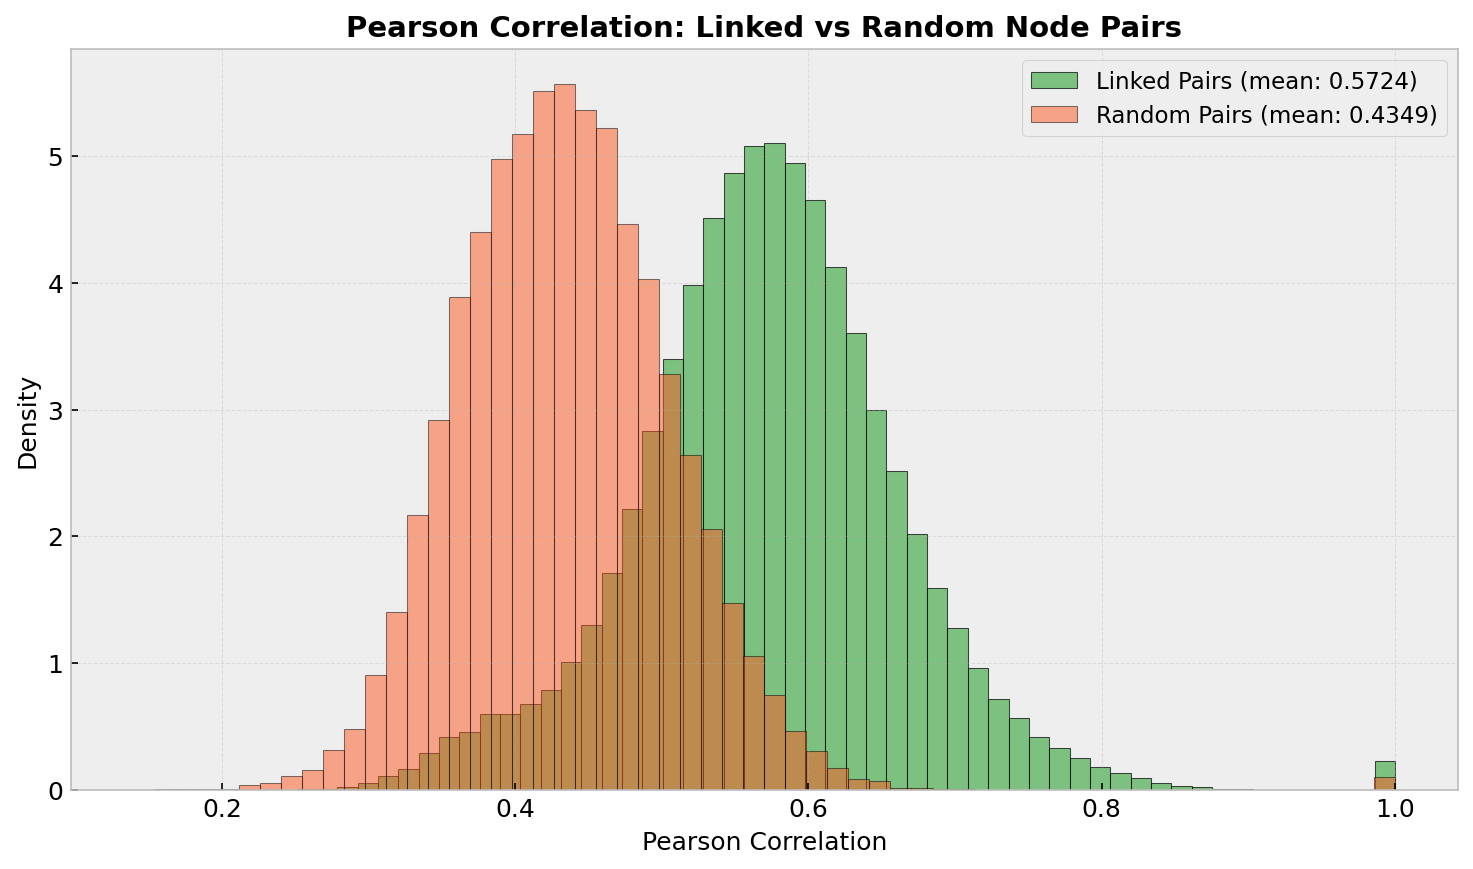
\includegraphics[width=0.75\textwidth]{figures/pearson-correlation-assortativity.png}
    \caption{Pearson correlation distribution: linked vs. random node pairs.}
    \label{fig:pearson-assort}
\end{figure}

\begin{figure}[H]
    \centering
    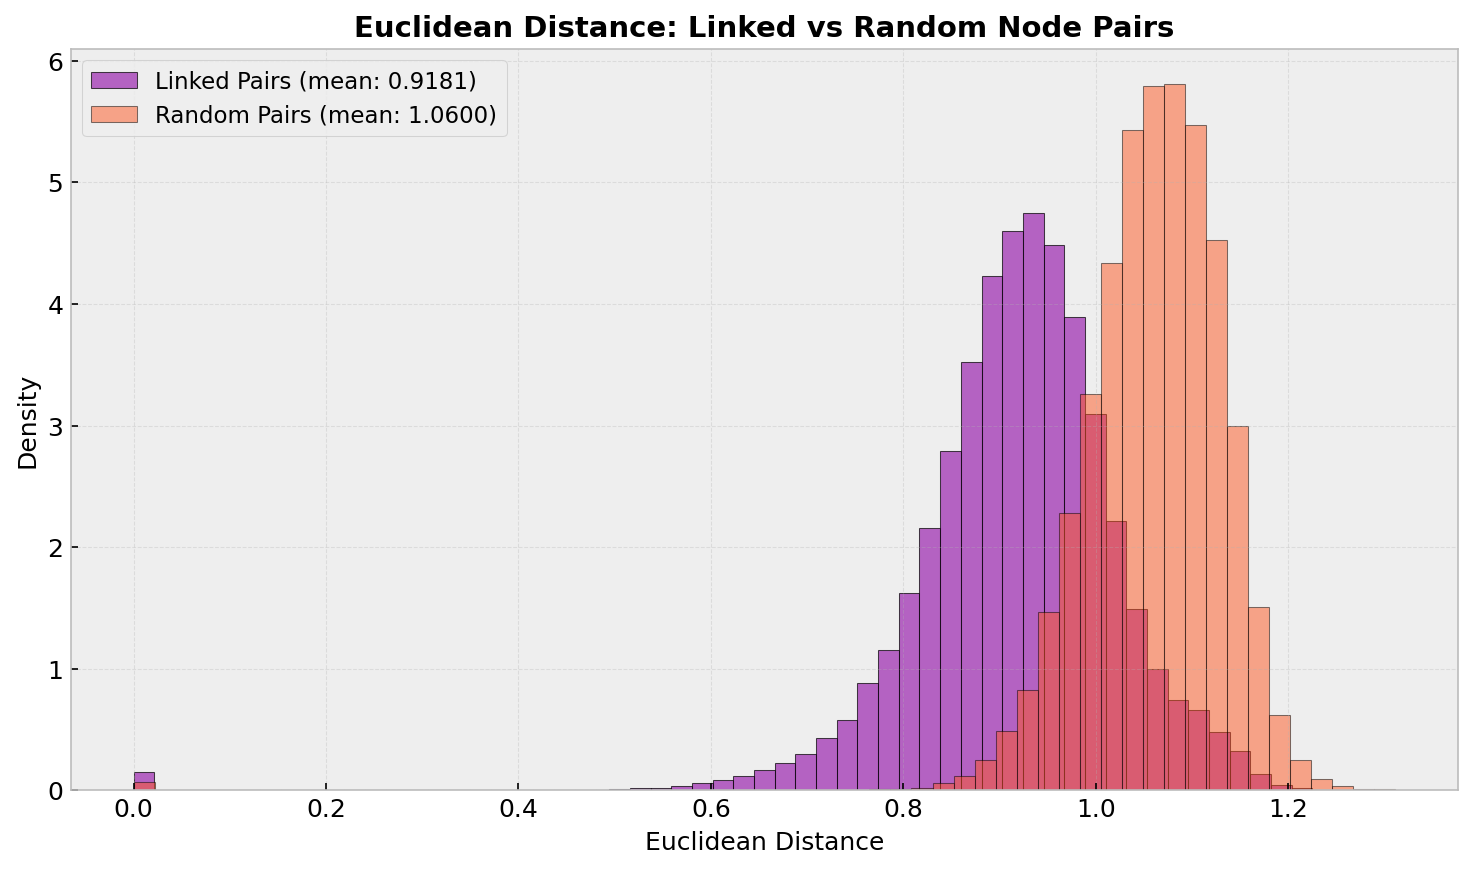
\includegraphics[width=0.75\textwidth]{figures/euclidean-distance-assortativity.png}
    \caption{Euclidean distance distribution: linked vs. random node pairs.}
    \label{fig:euclidean-assort}
\end{figure}

Table~\ref{tab:topic-link} summarises the topic-link assortativity results across all three metrics.

\begin{table}[htbp]
\centering
\caption{Topic-link assortativity summary across all three embedding metrics.}
\label{tab:topic-link}
\begin{tabular}{lccccc}
\toprule
\textbf{Metric} & \textbf{Linked Mean} & \textbf{Linked Std} & \textbf{Random Mean} & \textbf{Random Std} & \textbf{Diff} \\
\midrule
Cosine Similarity   & 0.5726 & 0.0901 & 0.4352 & 0.0724 & $+0.1374$ \\
Pearson Correlation & 0.5724 & 0.0902 & 0.4349 & 0.0725 & $+0.1375$ \\
Euclidean Distance  & 0.9181 & 0.1089 & 1.0600 & 0.0773 & $-0.1419$ \\
\bottomrule
\end{tabular}
\end{table}

\subsection{Community Detection Results}

Community detection using Louvain and Infomap algorithms reveals meaningful topical clusters in the graph.

\begin{figure}[H]
    \centering
    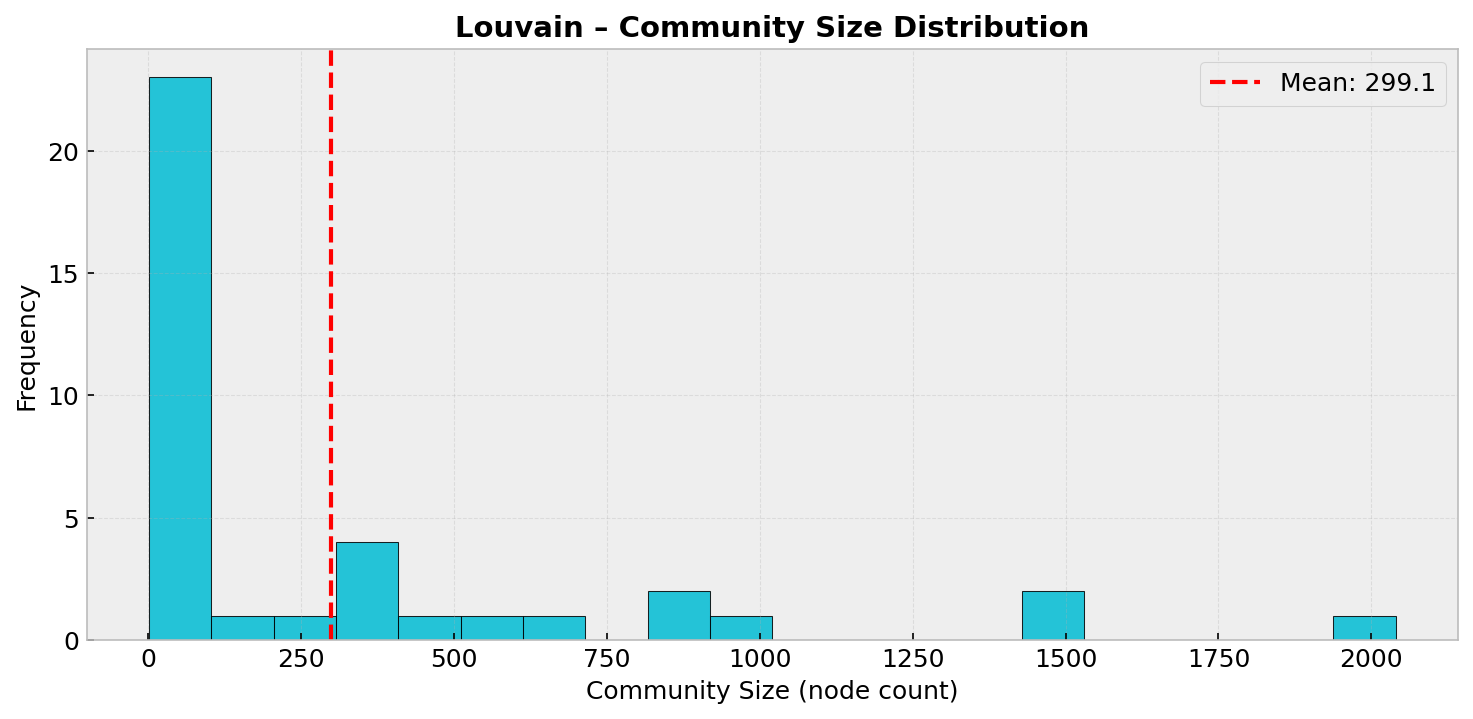
\includegraphics[width=0.75\textwidth]{figures/community-size-distribution-louvain.png}
    \caption{Louvain community size distribution (mean community size: 299.1 nodes).}
    \label{fig:louvain-communities}
\end{figure}

\begin{figure}[H]
    \centering
    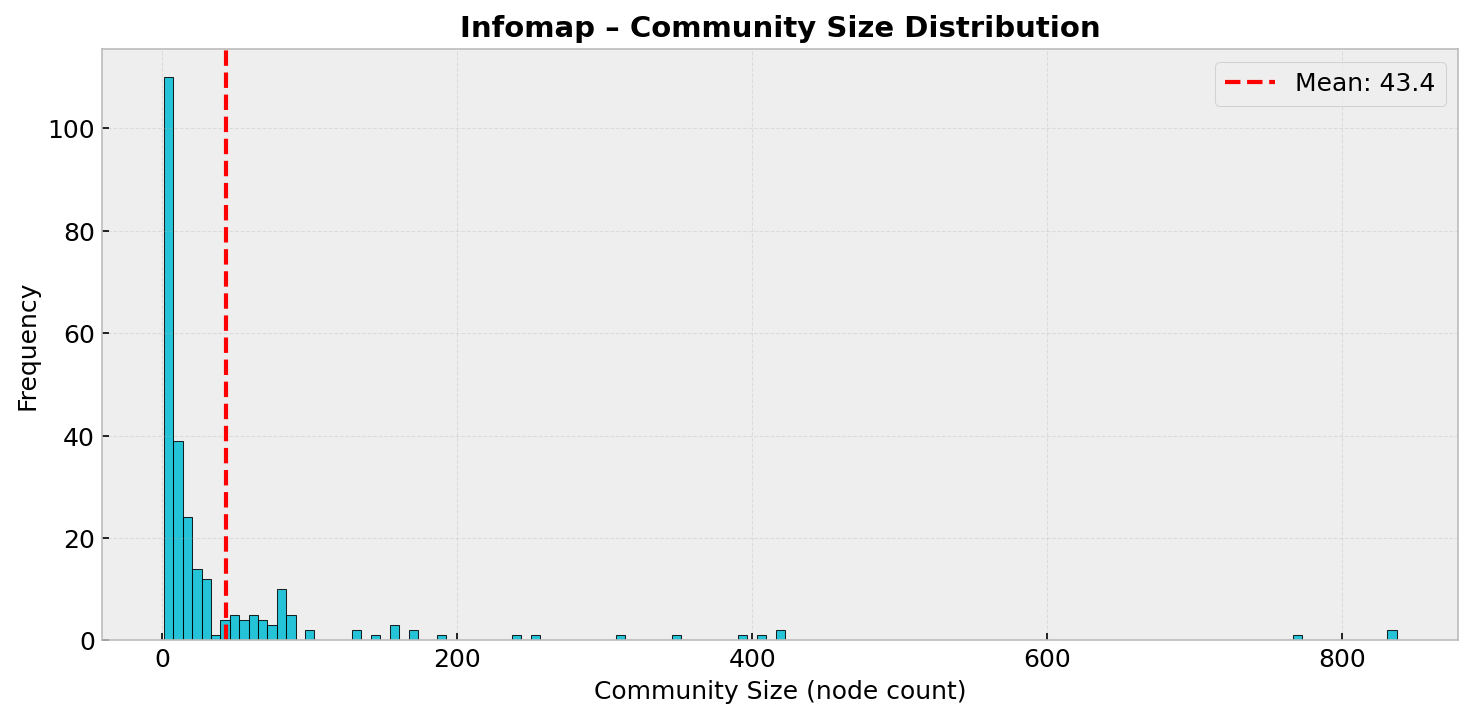
\includegraphics[width=0.75\textwidth]{figures/community-size-distribution-infomap.png}
    \caption{Infomap community size distribution (mean community size: 43.4 nodes).}
    \label{fig:infomap-communities}
\end{figure}

\begin{table}[htbp]
\centering
\caption{Community detection comparison: Louvain vs. Infomap.}
\label{tab:community-results}
\begin{tabular}{lrr}
\toprule
\textbf{Metric} & \textbf{Louvain} & \textbf{Infomap} \\
\midrule
Modularity             & 0.6476 & 0.5998 \\
Number of communities  & 38     & 262    \\
Max community size     & 2,040  & 837    \\
Mean community size    & 299.13 & 43.39  \\
Median community size  & 3      & 11     \\
\bottomrule
\end{tabular}
\end{table}

To validate that detected communities correspond to semantically coherent groups, Figure~\ref{fig:sim-dist} compares the cosine similarity of intra-community edges against inter-community edges.

\begin{figure}[H]
    \centering
    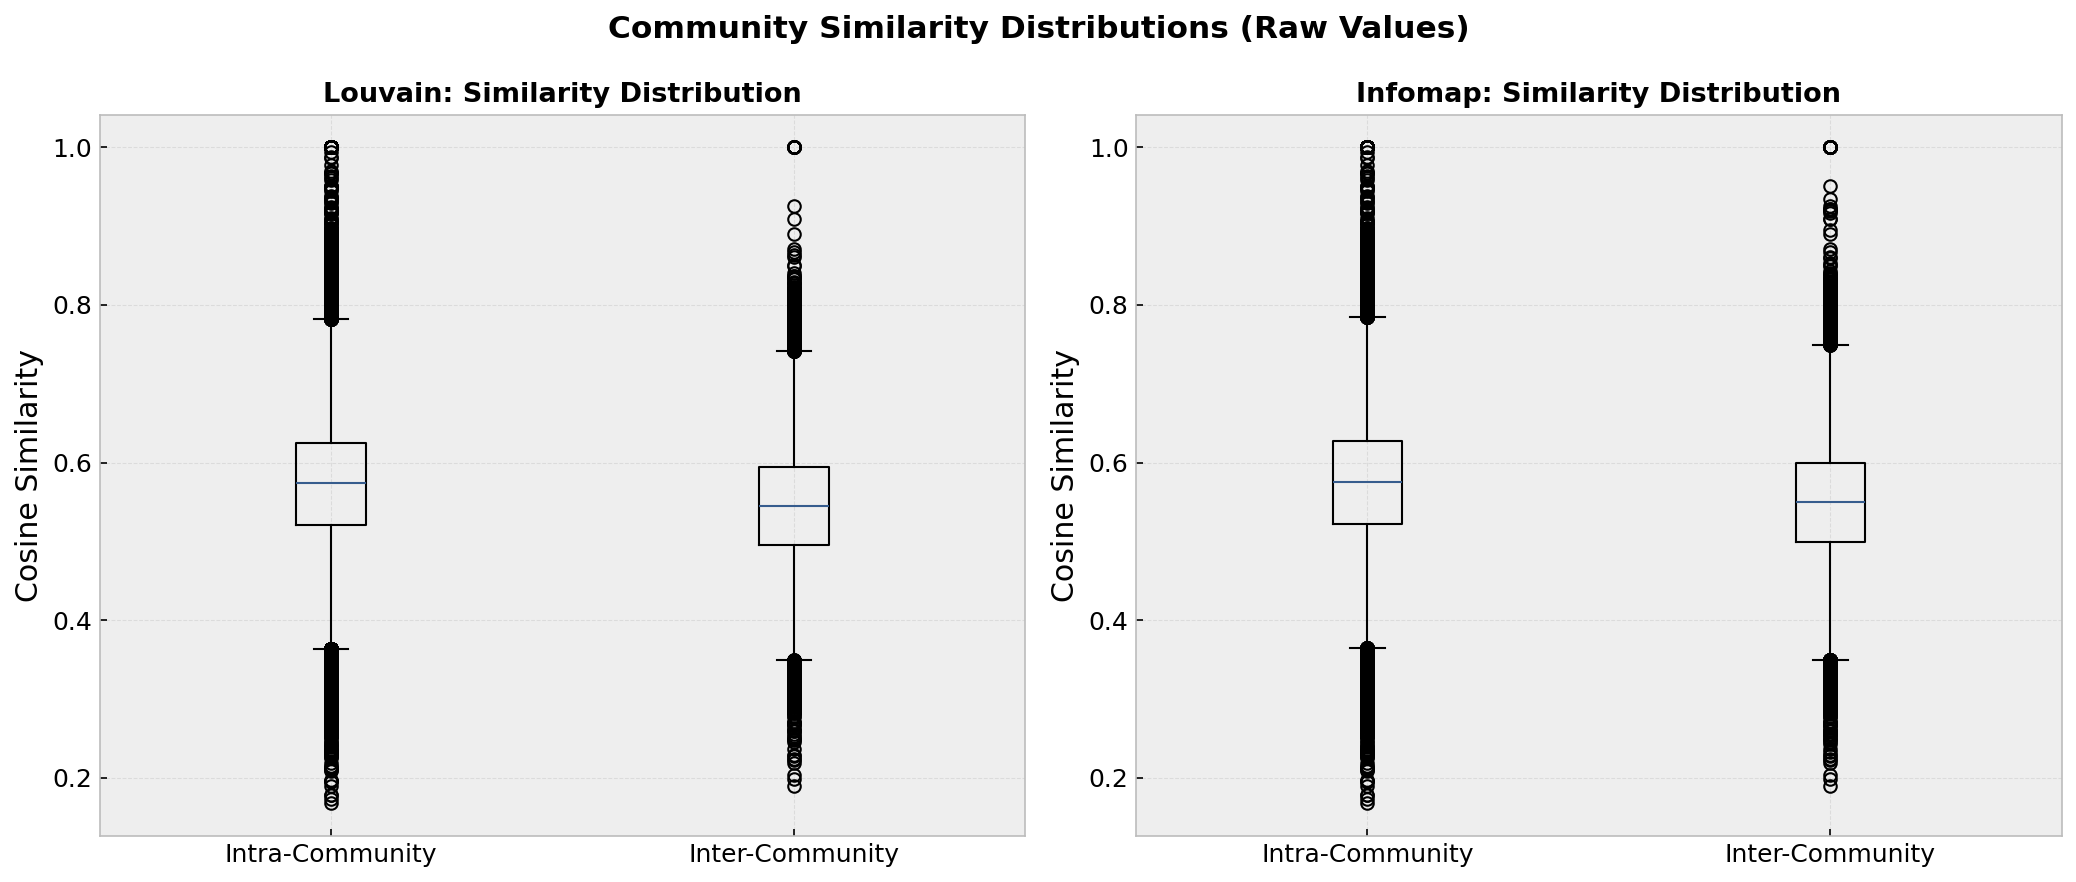
\includegraphics[width=0.75\textwidth]{figures/similarity-distributions.png}
    \caption{Intra-community vs. inter-community cosine similarity: Louvain (left) and Infomap (right).}
    \label{fig:sim-dist}
\end{figure}

\begin{table}[htbp]
\centering
\caption{Average cosine similarity: intra-community vs. inter-community edges.}
\label{tab:sim-community}
\begin{tabular}{lccc}
\toprule
\textbf{Algorithm} & \textbf{Intra-Community} & \textbf{Inter-Community} & \textbf{Difference} \\
\midrule
Louvain & 0.5729 & 0.5435 & $+0.0293$ \\
Infomap & 0.5748 & 0.5480 & $+0.0268$ \\
\bottomrule
\end{tabular}
\end{table}

Both algorithms confirm that the graph possesses meaningful community structure. Louvain produces a small number of large communities (mean $\approx$299 nodes), while Infomap finds many smaller, finer-grained communities (mean $\approx$43 nodes). Despite the difference in granularity, both algorithms agree on the key finding: nodes within the same community share consistently higher cosine similarity than nodes in different communities, validating the structural partitioning.

\subsection{GCN Baseline Link Prediction Results}

The first GNN experiments were conducted using a Graph Convolutional Network (GCN) baseline for the link prediction task.

\begin{table}[htbp]
\centering
\caption{GCN training dynamics with early stopping.}
\label{tab:gcn-results}
\begin{tabular}{rrrr}
\toprule
\textbf{Epoch} & \textbf{Loss} & \textbf{Val AUC} & \textbf{Notes} \\
\midrule
10 & 0.6356 & 0.8802 & \\
20 & 0.6059 & 0.8780 & \\
27 & --     & 0.8805 & Early stopped (Best Val AUC) \\
\midrule
\textbf{Test AUC (final)} & \multicolumn{3}{r}{\textbf{0.8653}} \\
\bottomrule
\end{tabular}
\end{table}

The GCN model rapidly achieves strong validation performance by epoch 10. With early stopping implemented, the model halts training at epoch 27, preventing the severe overfitting observed in extended 100-epoch runs. This baseline achieves a final Test AUC of 0.8653, demonstrating that topological learning alone provides a strong starting point.

The final test AUC of \textbf{0.8653} establishes a solid baseline for the link prediction task.

\subsection{Recommendation System Results}

A content-based recommendation system combining BGE-M3 embeddings and SVD-based Node2Vec was evaluated on 10 broad CS topic queries (Report-5).

\begin{table}[htbp]
\centering
\footnotesize
\caption{Sample recommendation results for broad topic queries.}
\label{tab:recommendation-results}
\begin{tabular}{lllr}
\toprule
\textbf{Query} & \textbf{Top-1 Recommendation} & \textbf{Similarity} & \textbf{Category} \\
\midrule
Natural Language Processing & Machine Translation & 0.731 & NLP \\
Operating System & History of Operating Systems & 0.789 & Systems \\
Programming Language & Compiler & 0.769 & PL \\
Database & Database Design & 0.737 & Data \\
Cloud Computing & Cloud Storage & 0.772 & Distributed \\
World Wide Web & Line Mode Browser & 0.729 & Web \\
Adversarial Machine Learning & AlgoSec & 0.800 & Security* \\
Brownout (Software Eng.) & Belady's Anomaly & 0.823 & Systems* \\
Computer and Network Surveillance & Cyber Spying & 0.705 & Security \\
Quantum Programming & Cloud-based Quantum Computing & 0.726 & Quantum \\
\bottomrule
\end{tabular}
\end{table}

*Note: Some queries (Adversarial ML, Brownout) return articles from adjacent topic clusters due to the structural signal from Node2Vec.

\subsection{Quantitative Evaluation}

Table~\ref{tab:quantitative-eval} presents the quantitative evaluation of the recommendation system on held-out test edges.

\begin{table}[htbp]
\centering
\caption{Recommendation system quantitative evaluation.}
\label{tab:quantitative-eval}
\begin{tabular}{lr}
\toprule
\textbf{Metric} & \textbf{Value} \\
\midrule
Test edges evaluated & 63,106 \\
Hits@1 rate & 1.70\% (1,075/63,106) \\
Hits@10 rate & 11.49\% (7,249/63,106) \\
MRR (Mean Reciprocal Rank) & 0.0548 \\
Random Hit@10 baseline & 0.086\% \\
Improvement vs. random & $\approx$ 134$\times$ \\
\bottomrule
\end{tabular}
\end{table}

The combined BGE-M3 + Node2Vec system achieves a Hits@10 rate of 11.49\%, representing a \textbf{134$\times$ improvement} over random recommendation. The MRR of 0.0548 indicates that the average test neighbor appears at rank $\approx$18.

\section{Summary and Discussion}

The results obtained to date demonstrate the feasibility of the proposed approach:

\begin{itemize}
    \item The Custom-WikiCS graph exhibits clear power-law degree distribution and meaningful community structure, confirming that Wikipedia's hyperlink structure encodes topical relationships
    \item Linked article pairs are significantly more similar (cosine: 0.5726 vs. 0.4352 random), validating the hypothesis that hyperlinks correlate with semantic similarity
    \item The GCN baseline achieves Test AUC = 0.8653 with early stopping, establishing a solid baseline for link prediction
    \item The recommendation system achieves 134$\times$ above random baseline, confirming that combined embeddings capture both semantic and structural signals
\end{itemize}

Areas requiring further investigation include:
\begin{itemize}
    \item GAT implementation and comparison against GCN baseline
    \item Early stopping and regularization strategies
    \item LLM-based hierarchical path organization (not yet implemented)
    \item Ablation studies on embedding combination strategies
\end{itemize}
